\documentclass[a4paper]{article} 
\usepackage[english]{babel} 
\usepackage[utf8x]{inputenc} 
\usepackage[T1]{fontenc} 
\usepackage{amsmath,amssymb,ragged2e,graphicx,float} 
\usepackage[a4paper,top=3cm,bottom=2cm,left=3cm,right=3cm,marginparwidth=1.75cm]{geometry} 
\begin{document} 
Recall that for a 2-link kinematic model there are 4 \emph{DOF} (i.e., \emph{SE}(2) $\times$ \emph{SE}(2) - constraints on $x,y$ at the joint = 4 \emph{DOF}). More specifically, the system can be completely defined by the location and orientation of a system's body frame (i.e., its \emph{position}) and the variables that reflects the relative placement of the component rigid bodies (i.e., its \emph{shape}). As seen in Figure \ref{fig:kinematics}B, the position of this system can be the \emph{SE}(2) location and orientation of the body frame and the shape is the orientation of the two links relative to each other ($\theta \in \mathbb{R}$).

When calculating the velocity of a frame that is not attached to the rigid body (as is the case when dealing with the center of gravity frame) it is often simpler to construct the velocity of the attached frames and then construct a transform to move the velocity back towards the disassociated frame. In order for this transform to work, it must be a function of the system's shape parameters. In fact, when choosing any generalized coordinate frames, any choice -- either attached to the rigid body or not -- is an acceptable choice as long as there exists a transformation element that is a function of the shape parameter such that the total configuration is still defined by the position and orientation of the frame and the shape parameter. It is therefore often convenient to choose an attached body frame to calculate all relative velocities only to transform back into the global (and often more difficult to derive) coordinate frame. As an example, assume that we chose the frame \emph{$g_2$} to be the coordinate frame. The total body velocity ($\xi$) is then defined as:

\begin{equation}\label{eq:totalbodyvelocity}
\xi 
=
\begin{bmatrix}
I_3  & 0^{3\times2}
\end{bmatrix}
=
\begin{bmatrix}
\xi \\
\dot{r}
\end{bmatrix}
\end{equation}

\begin{figure}[H]
\centering
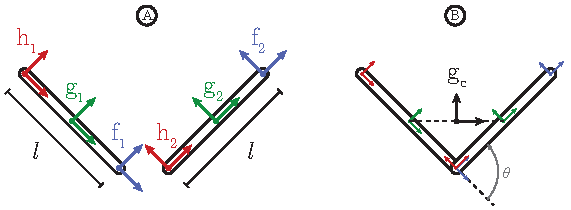
\includegraphics{Figure1}
\caption{Two-link model with frames on the proximal, middle, and distal ends of each link (A). Overall body from is calculated as the frame of reference of the center of mass, \emph{$g_{c}$} (B).}\label{fig:kinematics}
\end{figure}

\begin{figure}[H]
\centering
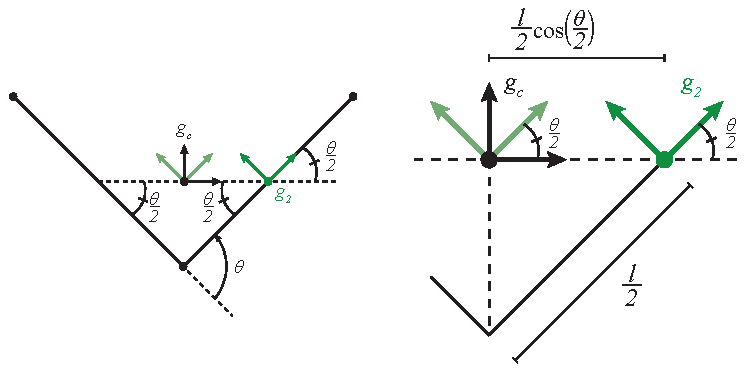
\includegraphics{Figure2}
\caption{Calculation of the overall body frame in relation to frame \emph{$g_2$}. For the sake of simplicity, the link lengths were set to the same value, \emph{l}, so that the angle generated between \emph{$g_{c}$} and \emph{$g_{2}$} (when instantaneously superimposed) will become half of the independent variable angle, $\theta$ (Left).}\label{fig:overallbodyframe}
\end{figure}

\end{document}